\documentclass[9pt,aspectratio=169,xcolor=table]{beamer}

%~~~~~~~~~~~~~~~~~~~~~~~~~~~~~~~~~~~~~~~~~~~~~~~~~~~~~~~~~~~~~~~~~~~~~~~~~~~~~~
% Use roboto Font (recommended)
\usepackage[sfdefault]{roboto}
\usepackage[utf8]{inputenc}
\usepackage[T1]{fontenc}
%~~~~~~~~~~~~~~~~~~~~~~~~~~~~~~~~~~~~~~~~~~~~~~~~~~~~~~~~~~~~~~~~~~~~~~~~~~~~~~

%~~~~~~~~~~~~~~~~~~~~~~~~~~~~~~~~~~~~~~~~~~~~~~~~~~~~~~~~~~~~~~~~~~~~~~~~~~~~~~
% Define where theme files are located. ('/styles')
\usepackage{styles/fluxmacros}
\usefolder{styles}
% Use Flux theme v0.1 beta
% Available style: asphalt, blue, red, green, gray
\usetheme[style=hunter]{flux}
%~~~~~~~~~~~~~~~~~~~~~~~~~~~~~~~~~~~~~~~~~~~~~~~~~~~~~~~~~~~~~~~~~~~~~~~~~~~~~~

%~~~~~~~~~~~~~~~~~~~~~~~~~~~~~~~~~~~~~~~~~~~~~~~~~~~~~~~~~~~~~~~~~~~~~~~~~~~~~~
% Extra packages
\usepackage{booktabs}
\usepackage{colortbl}
\usepackage{ragged2e}
\usepackage{amssymb}
\usepackage{multirow}
\usepackage{tikz}
\usetikzlibrary{arrows.meta, positioning, fit, backgrounds, calc, decorations.pathreplacing}
\setbeamertemplate{itemize items}[square]
\usepackage[scaled=.8]{beramono}
\usepackage{listings}
\usepackage{styles/lstlangarm}
\usepackage{array}
\definecolor{bgcolor}{HTML}{F2E9E9}
% lstlangarm.sty references \color{mauve} for string literals but never defines
% it -- only fires when a listing contains a string. Define it here.
\definecolor{mauve}{rgb}{0.58,0,0.82}
% lstlangarm's C style sets commentstyle=green!20, which is unreadable on the
% pink listing background. Darken it globally.
\lstset{commentstyle=\color{green!45!black}}
% ragged-right fixed-width column -- must be defined in the preamble, never
% inside a frame (\newcolumntype's #1 breaks beamer's frame scanner)
\newcolumntype{R}[1]{>{\RaggedRight\arraybackslash}p{#1}}
%~~~~~~~~~~~~~~~~~~~~~~~~~~~~~~~~~~~~~~~~~~~~~~~~~~~~~~~~~~~~~~~~~~~~~~~~~~~~~~
% Table striping: odd rows white, even rows very light gray.
% Needs \documentclass[...,xcolor=table]{beamer} (beamer loads xcolor itself,
% so the option must go on the class, not \usepackage).
\definecolor{stripe}{gray}{0.94}
% \striped makes body rows alternate white, gray, white, ... starting white.
% \rowcolors counts from the first coloured body row; the header is not counted.
\newcommand{\striped}{\rowcolors{1}{white}{stripe}}
%~~~~~~~~~~~~~~~~~~~~~~~~~~~~~~~~~~~~~~~~~~~~~~~~~~~~~~~~~~~~~~~~~~~~~~~~~~~~~~

%~~~~~~~~~~~~~~~~~~~~~~~~~~~~~~~~~~~~~~~~~~~~~~~~~~~~~~~~~~~~~~~~~~~~~~~~~~~~~~
% TikZ block styles -- matches ch1/ch2
% Colour variables are named identically in the book's stm32primer.tex, so any
% tikzpicture using only the \tikzset{...} styles below can be copied verbatim
% between slides and book. Only the \definecolor/\colorlet VALUES differ: the
% book is printed, so it keeps every stroke pure black with muted fills. These
% slides are projected, so both fill AND stroke are bright and saturated to
% grab attention -- see stm32primer.tex for the print palette.
\definecolor{blkfill}{HTML}{DDEEDD}
\definecolor{blkline}{HTML}{355E3B}
\definecolor{accentfill}{HTML}{FFE0B2}
\definecolor{accentline}{HTML}{E65100}
\definecolor{memfill}{HTML}{DFF5DA}
\definecolor{memline}{HTML}{2E7D32}
\definecolor{cellfill}{HTML}{FFFFFF}
\definecolor{cellline}{HTML}{424242}
\definecolor{bitmaskfill}{HTML}{DCEBFF}
\definecolor{bitmaskline}{HTML}{1565C0}
\definecolor{bithitfill}{HTML}{FFE0B2}
\definecolor{bithitline}{HTML}{E65100}
\tikzset{
  blk/.style   = {rectangle, rounded corners=2pt, draw=blkline, fill=blkfill,
                  thick, align=center, font=\small, minimum height=9mm, inner sep=3pt},
  cpublk/.style= {rectangle, rounded corners=2pt, draw=accentline, fill=accentfill,
                  thick, align=center, font=\small\bfseries, minimum height=9mm, inner sep=3pt},
  memblk/.style= {rectangle, rounded corners=2pt, draw=memline, fill=memfill,
                  thick, align=center, font=\small, minimum height=9mm, inner sep=3pt},
  cell/.style  = {rectangle, draw=cellline, fill=cellfill, align=center,
                  font=\small\ttfamily, minimum height=7mm, inner sep=2pt},
  bitcell/.style={rectangle, draw=cellline, fill=cellfill, thick,
                  minimum width=5.4mm, minimum height=5.4mm, inner sep=0pt,
                  font=\scriptsize\ttfamily, anchor=center},
  bitmask/.style={bitcell, fill=bitmaskfill, draw=bitmaskline},
  bithit/.style ={bitcell, fill=bithitfill, draw=bithitline, font=\scriptsize\ttfamily\bfseries},
  rowlab/.style ={font=\scriptsize, text=Gray, anchor=east},
  oplab/.style  ={font=\scriptsize\itshape, text=Gray, anchor=west},
  lbl/.style   = {font=\scriptsize, text=Gray},
  flow/.style  = {-{Stealth[length=2mm]}, thick, draw=blkline},
  busline/.style={thick, draw=cellline},
}
% NOTE (theme quirks -- all fail SILENTLY, always page through the PDF):
%  - a second \\ inside a nested {...} group in a TikZ node breaks parsing
%  - {\small ...} wrapped around a nested itemize eats the frame title + list
%  - \usebeamercolor on a [plain] frame falls through to an unstyled default
%  - \newcolumntype inside a frame breaks beamer's frame scanner
%  - lstlisting needs \begin{frame}[fragile]
%  - a TikZ picture wider than its column silently overflows into neighbours
%~~~~~~~~~~~~~~~~~~~~~~~~~~~~~~~~~~~~~~~~~~~~~~~~~~~~~~~~~~~~~~~~~~~~~~~~~~~~~~

%%%%%%%%%%%%%%%%%%%%%%%%%%%%%%%%%%%
%% BEGIN CONDITIONAL COMPILATION %%
%%%%%%%%%%%%%%%%%%%%%%%%%%%%%%%%%%%
\newif\ifwebex
%\webextrue % uncomment to generate section separator
\ifwebex
\AtBeginSection[]{
  \begin{frame}
  \vfill
  \centering
  \begin{beamercolorbox}[sep=8pt,center,shadow=true,rounded=true]{title}
    \usebeamerfont{title}\insertsectionhead\par%
  \end{beamercolorbox}
  \vfill
  \end{frame}
}
\else
\AtBeginSection[]
{
{
    \setbeamercolor{background canvas}{bg=yellow!10}
    \begin{frame}[plain]
        \frametitle{Table of Contents}
        \tableofcontents[currentsection]
    \end{frame}
}
}
\fi
%%%%%%%%%%%%%%%%%%%%%%%%%%%%%%%%%%%
%% END CONDITIONAL COMPILATION   %%
%%%%%%%%%%%%%%%%%%%%%%%%%%%%%%%%%%%

%~~~~~~~~~~~~~~~~~~~~~~~~~~~~~~~~~~~~~~~~~~~~~~~~~~~~~~~~~~~~~~~~~~~~~~~~~~~~~~
% Information
\title{Registers and Shift Registers}
\subtitle{\emph{Contemporary Digital Electronic Systems} --- Chapter 11}
\author{Mun\'{i}m Zabidi}
\institute{\color{primary}Faculty of Electrical Engineering, Universiti Teknologi Malaysia}
\date{\today}
\titlegraphic{assets/logoutmwhite.png}
\graphicspath{{.}{../fig/}}
%~~~~~~~~~~~~~~~~~~~~~~~~~~~~~~~~~~~~~~~~~~~~~~~~~~~~~~~~~~~~~~~~~~~~~~~~~~~~~~

\newcommand{\figh}[2]{\includegraphics[height=#1\textheight]{#2}}

\begin{document}

\titlepage

%===============================================================================
\section{Why This Chapter}
%===============================================================================

\begin{frame}{Why This Chapter Matters}
  \begin{columns}[c]
  \begin{column}{.47\textwidth}
    A flip-flop stores one bit. In practice we store, move and transform groups of bits: a 32-bit word, a 16-bit instruction, a stream of serial data. Grouping flip-flops into \alert{registers}, and especially \alert{shift registers}, gives building blocks for serial links, pipelines and every sequential module that follows. Two kinds of counter appear here, shift-register and accumulator counters; flip-flop-based counters follow in Chapter 12.
  \end{column}
  \begin{column}{.51\textwidth}
    \begin{block}{After this chapter, you can:}
    {\small
    \begin{enumerate}\itemsep2pt
      \item Draw an $n$-bit parallel-load register and describe its controls.
      \item Distinguish SISO, SIPO, PISO and PIPO shift registers and give an application of each.
      \item Design a shift register with load, shift-left, shift-right and hold modes.
      \item Explain serial--parallel conversion.
      \item Recognise ring and Johnson counters as shift-register configurations.
    \end{enumerate}}
    \end{block}
  \end{column}
  \end{columns}
\end{frame}

\begin{frame}{An Opening Question}
  \leavevmode\vspace{4mm}
  \begin{center}
  \fbox{\parbox{.78\textwidth}{\centering\vspace{2mm}
  \large How does a laptop talk to a USB device through a connector with only a handful of wires, when thousands of bytes must be exchanged?
  \vspace{2mm}}}
  \end{center}
  \vspace{4mm}
  The key idea is \alert{serial--parallel conversion} with shift registers.
\end{frame}

%===============================================================================
\section{Data Registers}
%===============================================================================

\begin{frame}{Basic Data Register}
  \begin{columns}[c]
  \begin{column}{.5\textwidth}
    \centering
    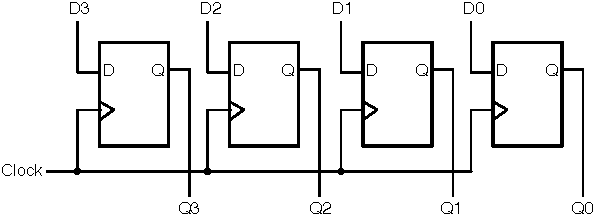
\includegraphics[width=\textwidth]{reg4basic_sc}
  \end{column}
  \begin{column}{.48\textwidth}
    \centering
    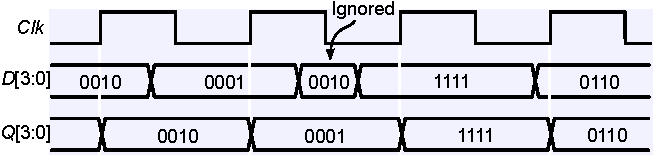
\includegraphics[width=\textwidth]{reg4basic_td}
  \end{column}
  \end{columns}
  \begin{itemize}\small\itemsep3pt
    \item A register holds binary information while it awaits processing or after it is produced.
    \item Four D flip-flops share one clock: on every rising edge the $D$ inputs are stored. Most registers use positive-edge-triggered D flip-flops.
  \end{itemize}
\end{frame}

\begin{frame}{Register with Clear}
  \begin{columns}[c]
  \begin{column}{.5\textwidth}
    \centering
    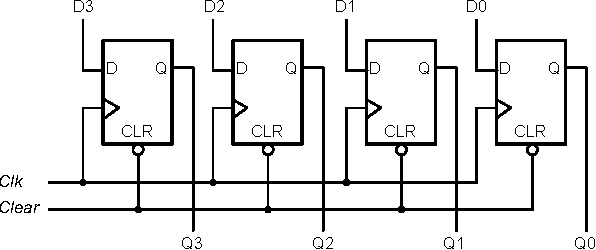
\includegraphics[width=\textwidth]{reg4clr_sc}
  \end{column}
  \begin{column}{.48\textwidth}
    \centering
    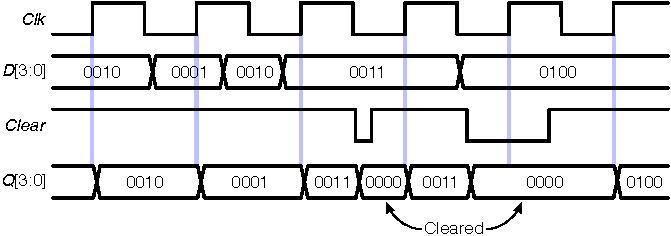
\includegraphics[width=\textwidth]{reg4clr_td}
  \end{column}
  \end{columns}
  \begin{itemize}\small\itemsep3pt
    \item Registers must start from a known state (start-up, error recovery), so they get a reset input.
    \item An active-low, \alert{asynchronous} clear forces all flip-flops to 0 immediately, with no clock pulse needed.
  \end{itemize}
\end{frame}

\begin{frame}{Register with Load Enable}
  \begin{columns}[c]
  \begin{column}{.5\textwidth}
    \centering
    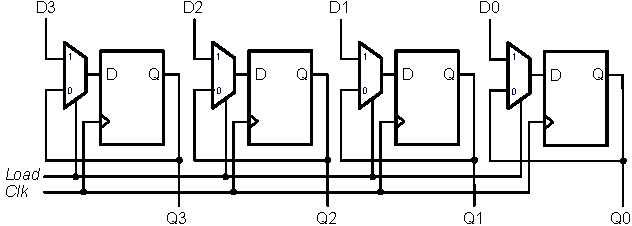
\includegraphics[width=\textwidth]{reg4load_sc}
  \end{column}
  \begin{column}{.48\textwidth}
    \centering
    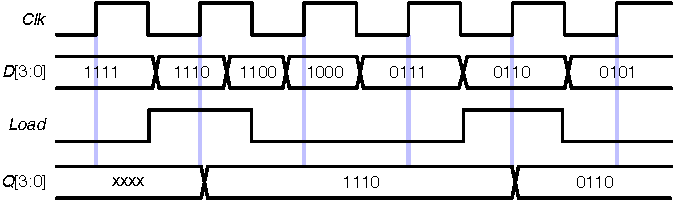
\includegraphics[width=\textwidth]{reg4load_td}
  \end{column}
  \end{columns}
  \begin{itemize}\small\itemsep3pt
    \item A mux at each flip-flop input, controlled by \texttt{Load}.
    \item \texttt{Load} = 1: new data enters on the next rising edge. \texttt{Load} = 0: the flip-flop's own output is fed back, so the register holds its value.
    \item The register updates only when new data is available.
  \end{itemize}
\end{frame}

%===============================================================================
\section{Shift Registers}
%===============================================================================

\begin{frame}{Four Types of Shift Register}
  \begin{columns}[c]
  \begin{column}{.5\textwidth}
    \begin{itemize}\small\itemsep3pt
      \item A shift register passes data from stage to stage on each clock pulse: storage, transfer, delay, serial--parallel conversion.
      \item \alert{SISO}: serial in, serial out.
      \item \alert{SIPO}: serial in, parallel out.
      \item \alert{PISO}: parallel in, serial out.
      \item \alert{PIPO}: parallel in, parallel out.
    \end{itemize}
  \end{column}
  \begin{column}{.48\textwidth}
    \centering\small
    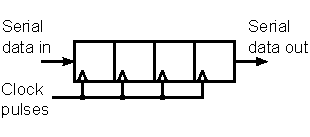
\includegraphics[height=.17\textheight]{sreg-siso}\hspace{2mm}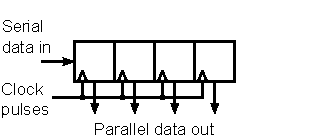
\includegraphics[height=.17\textheight]{sreg-sipo}\\
    SISO \hspace{.15\textwidth} SIPO\\[2mm]
    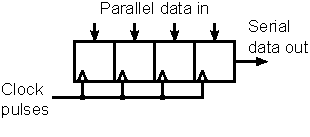
\includegraphics[height=.17\textheight]{sreg-piso}\hspace{2mm}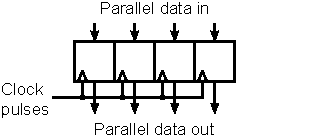
\includegraphics[height=.17\textheight]{sreg-pipo}\\
    PISO \hspace{.15\textwidth} PIPO
  \end{column}
  \end{columns}
\end{frame}

\begin{frame}{SISO and SIPO Logic Diagrams}
  \centering
  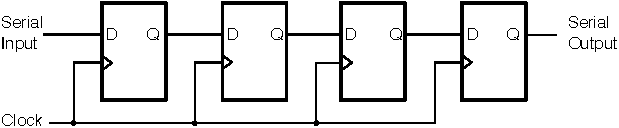
\includegraphics[height=.17\textheight]{siso}\\[1mm]{\scriptsize SISO}\\[2mm]
  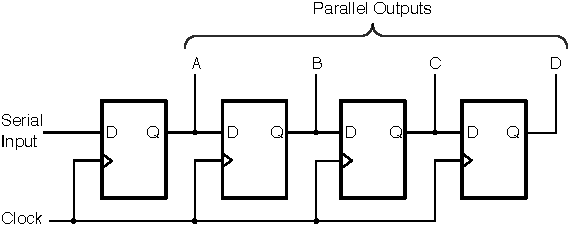
\includegraphics[height=.3\textheight]{sipo}\\[1mm]{\scriptsize SIPO}
  \begin{itemize}\small
    \item Both shift data one stage per clock. A SISO gives only the last bit; a SIPO exposes every stage.
  \end{itemize}
\end{frame}

\begin{frame}{SIPO Operation}
  \begin{columns}[c]
  \begin{column}{.4\textwidth}
    \centering
    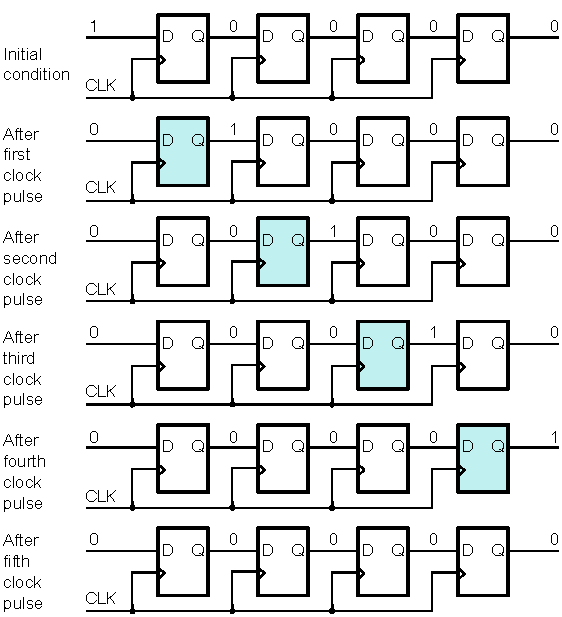
\includegraphics[height=.62\textheight]{sreg-anim}
  \end{column}
  \begin{column}{.58\textwidth}
    \begin{enumerate}\small\itemsep2pt
      \item Apply a bit to the serial input.
      \item Apply a clock pulse.
      \item The bit is stored in the first flip-flop.
      \item Every stage shifts one position right.
      \item Read the parallel outputs.
      \item Repeat until all bits are loaded.
    \end{enumerate}
    \centering
    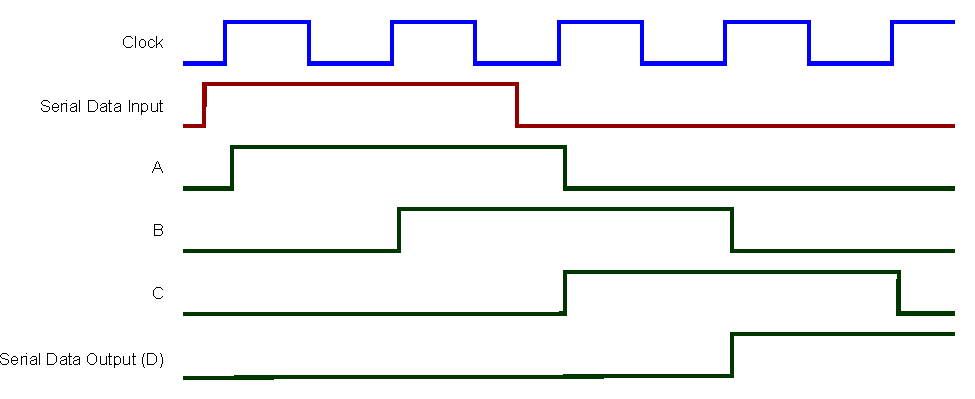
\includegraphics[width=.95\textwidth]{sreg_timing}
  \end{column}
  \end{columns}
\end{frame}

\begin{frame}{Example: Loading 1011 into a SIPO Register}
  \begin{columns}[c]
  \begin{column}{.5\textwidth}
    \small Stages $A, B, C, D$ ($A$ nearest the input), starting at 0000; input \texttt{1011}, MSB first.\\[2mm]
    \centering\small\striped
    \begin{tabular}{@{}c|c|cccc@{}}
      \toprule
      Pulse & In & $A$ & $B$ & $C$ & $D$ \\
      \midrule
      1 & 1 & 1 & 0 & 0 & 0 \\
      2 & 0 & 0 & 1 & 0 & 0 \\
      3 & 1 & 1 & 0 & 1 & 0 \\
      4 & 1 & 1 & 1 & 0 & 1 \\
      \bottomrule
    \end{tabular}
  \end{column}
  \begin{column}{.48\textwidth}
    \begin{itemize}\small\itemsep3pt
      \item After four pulses $ABCD = 1101$.
      \item Reading from $D$ (first bit in) to $A$ (last bit in) recovers \texttt{1011}.
    \end{itemize}
    \begin{block}{Uses}
      \small SISO: delay line. SIPO / PISO: serial--parallel interface. PIPO: temporary storage of a whole word.
    \end{block}
  \end{column}
  \end{columns}
\end{frame}

\begin{frame}{Shift Register with Enable}
  \centering
  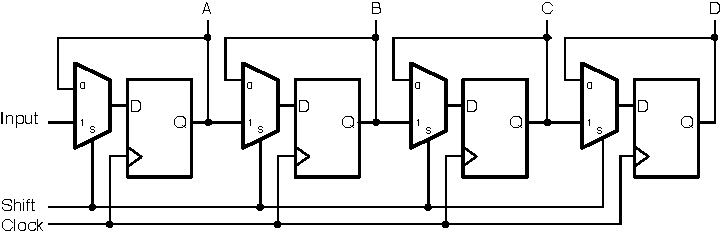
\includegraphics[width=.8\textwidth]{sipo-v2}
  \begin{itemize}\small\itemsep3pt
    \item A mux at each flip-flop input, controlled by a common \texttt{Shift} signal. \texttt{Shift} = 1: shift each clock. \texttt{Shift} = 0: no shifting.
    \item Larger muxes allow more input sources, including external data: the route to PISO and PIPO operation.
  \end{itemize}
\end{frame}

\begin{frame}{Universal Shift Register}
  \begin{columns}[c]
  \begin{column}{.4\textwidth}
    \centering
    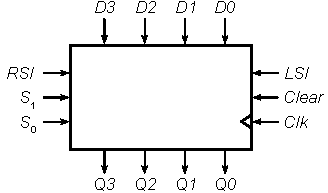
\includegraphics[width=.8\textwidth]{sreg4univ_top}\\[2mm]
    \small\striped
    \begin{tabular}{@{}cc|l@{}}
      \toprule
      $S_1$ & $S_0$ & Function \\
      \midrule
      0&0&Hold \\ 0&1&Shift left \\ 1&0&Shift right \\ 1&1&Load \\
      \bottomrule
    \end{tabular}
  \end{column}
  \begin{column}{.58\textwidth}
    \begin{itemize}\small\itemsep3pt
      \item Serial-to-serial, serial-to-parallel, parallel-to-serial, parallel-to-parallel; left and right shifts.
      \item Shift left: $Q_3 Q_2 Q_1 \leftarrow Q_2 Q_1 Q_0$, $Q_0 \leftarrow LSI$.
      \item Shift right: $Q_2 Q_1 Q_0 \leftarrow Q_3 Q_2 Q_1$, $Q_3 \leftarrow RSI$.
      \item Left shift is like multiplication by 2; right shift like division by 2.
    \end{itemize}
  \end{column}
  \end{columns}
\end{frame}

\begin{frame}{Universal Shift Register: Schematic and Timing}
  \centering
  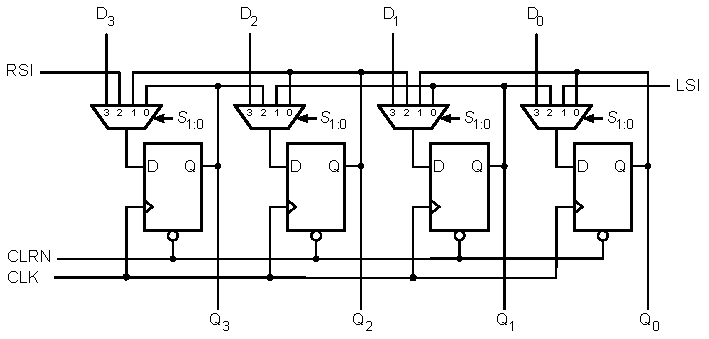
\includegraphics[height=.36\textheight]{sreg4univ_sc}\hspace{4mm}
  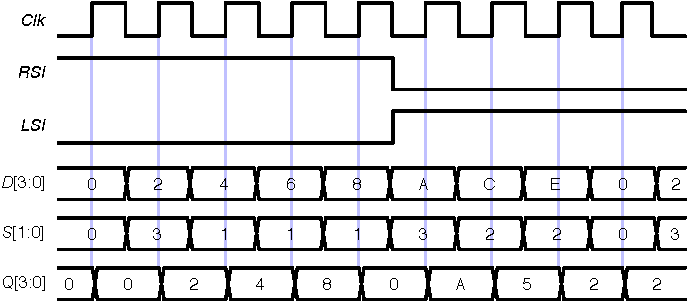
\includegraphics[height=.36\textheight]{sreg4univ_td}
\end{frame}

%===============================================================================
\section{Shift-Register Counters}
%===============================================================================

\begin{frame}{Ring Counter}
  \begin{itemize}\small\itemsep3pt
    \item The last stage feeds the first: a single 1 circulates. 4-bit sequence: $1000 \to 0100 \to 0010 \to 0001 \to 1000 \to \cdots$
    \item $n$ flip-flops give only $n$ valid states (versus $2^n$ for a binary counter), but each state is trivially decoded.
    \item It must be initialised: set one flip-flop and clear the rest (preset on the first, clear on the others), or detect all-zero and reload ($D_A = \overline{A}\,\overline{B}\,\overline{C}$).
  \end{itemize}
  \centering
  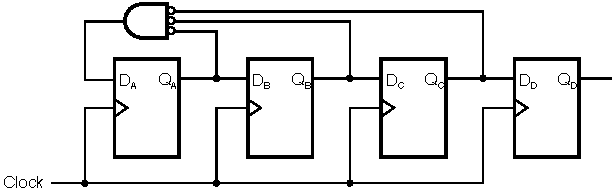
\includegraphics[height=.2\textheight]{ctr_ring_sch}\hspace{4mm}
  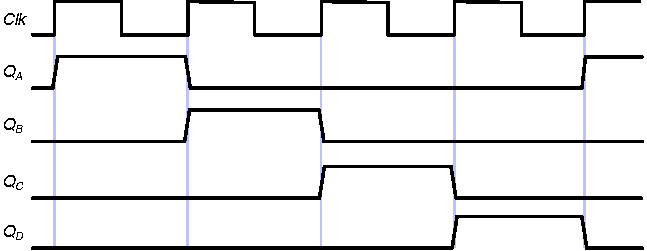
\includegraphics[height=.2\textheight]{ctr_ring_td}
\end{frame}

\begin{frame}{Johnson Counter}
  \begin{columns}[c]
  \begin{column}{.5\textwidth}
    \begin{itemize}\small\itemsep3pt
      \item Also called twisted-ring or M\"obius counter: feeds the \alert{inverted} last output to the first.
      \item $n$ flip-flops give $2n$ states.
      \item Only one bit changes per clock, and each state is easier to decode than a ring counter's.
      \item Uses $2n$ of $2^n$ states: invalid power-up states form separate loops and do not self-correct without added logic or a reset.
    \end{itemize}
    \centering
    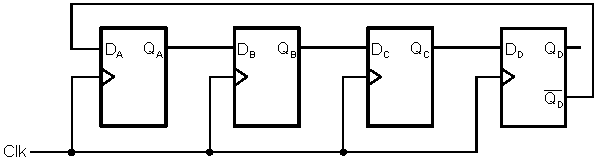
\includegraphics[width=.9\textwidth]{ctr_johnson_sch}
  \end{column}
  \begin{column}{.48\textwidth}
    \centering\scriptsize\striped
    \begin{tabular}{@{}c|cccc@{}}
      \toprule
      Clock & $A$ & $B$ & $C$ & $D$ \\
      \midrule
      0&0&0&0&0 \\ 1&1&0&0&0 \\ 2&1&1&0&0 \\ 3&1&1&1&0 \\
      4&1&1&1&1 \\ 5&0&1&1&1 \\ 6&0&0&1&1 \\ 7&0&0&0&1 \\ 8&0&0&0&0 \\
      \bottomrule
    \end{tabular}\\[1mm]
    {\small Back to 0000 after $2n = 8$ pulses.}
  \end{column}
  \end{columns}
\end{frame}

\begin{frame}{Johnson Counter: Timing}
  \centering
  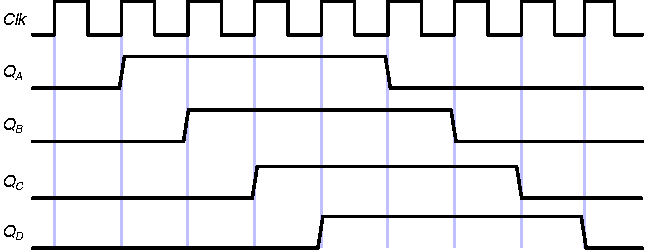
\includegraphics[height=.42\textheight]{ctr_johnson_td}
  \begin{itemize}\small
    \item Eight distinct states with one bit changing at each step, which helps reduce decoding errors.
  \end{itemize}
\end{frame}

\begin{frame}{Linear-Feedback Shift Register (LFSR)}
  \centering
  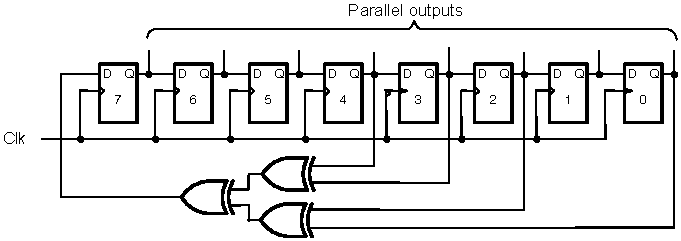
\includegraphics[width=.65\textwidth]{lfsr8bit}
  \begin{itemize}\small\itemsep3pt
    \item Selected stage outputs (the \alert{taps}) are XORed and fed back to the first stage.
    \item With the right taps, an $n$-bit LFSR cycles through all $2^n - 1$ non-zero states: a pseudo-random sequence (testing, cryptography, communications).
    \item 8 bits: taps 4, 3, 2, 0 give 255 states. The all-zero state is forbidden: it never changes.
  \end{itemize}
\end{frame}

\begin{frame}{LFSR Tap Table and Example}
  \begin{columns}[c]
  \begin{column}{.4\textwidth}
    \centering\tiny\striped
    \begin{tabular}{@{}crl@{}}
      \toprule
      Stages & Length & Taps \\
      \midrule
      2&3&1,0 \\ 3&7&1,0 \\ 4&15&1,0 \\ 5&31&2,0 \\ 6&63&1,0 \\ 7&127&1,0 \\
      8&255&4,3,2,0 \\ 9&511&4,0 \\ 10&1023&3,0 \\ 12&4095&6,4,1,0 \\ 16&65535&12,3,1,0 \\
      \bottomrule
    \end{tabular}
  \end{column}
  \begin{column}{.58\textwidth}
    \small Load \texttt{00000001}; $F = Q_4 \oplus Q_3 \oplus Q_2 \oplus Q_0$ enters $Q_7$.\\[1mm]
    \centering\scriptsize\striped
    \begin{tabular}{@{}c|cc|c@{}}
      \toprule
      Clock & State $Q_7 \dots Q_0$ & Dec & $F$ \\
      \midrule
      0 & 0000\,0001 & 1 & 1 \\ 1 & 1000\,0000 & 128 & 0 \\ 2 & 0100\,0000 & 64 & 0 \\ 3 & 0010\,0000 & 32 & 0 \\
      4 & 0001\,0000 & 16 & 1 \\ 5 & 1000\,1000 & 136 & 1 \\ 6 & 1100\,0100 & 196 & 1 \\
      \bottomrule
    \end{tabular}
  \end{column}
  \end{columns}
\end{frame}

%===============================================================================
\section{Accumulators}
%===============================================================================

\begin{frame}{Accumulator-Based Counters}
  \begin{columns}[c]
  \begin{column}{.4\textwidth}
    \centering
    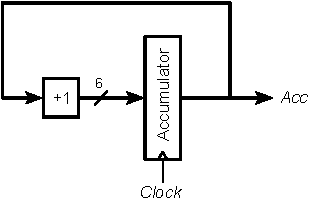
\includegraphics[width=.9\textwidth]{accum_basic}
  \end{column}
  \begin{column}{.58\textwidth}
    \centering
    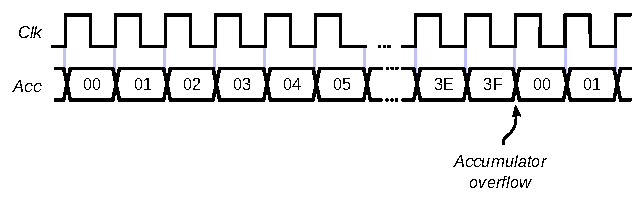
\includegraphics[width=.9\textwidth]{accum01td}
  \end{column}
  \end{columns}
  \begin{itemize}\small\itemsep3pt
    \item An \alert{accumulator} is a register whose output is fed back through combinational logic: results build up over clock cycles.
    \item A register plus an incrementer is a counter: this 6-bit one counts 00 to 3F and wraps to 00.
    \item Easy to design (register width sets the count size); speed is set mainly by the adder delay.
  \end{itemize}
\end{frame}

\begin{frame}{Resettable and Multifunction Counters}
  \begin{columns}[c]
  \begin{column}{.33\textwidth}
    \centering
    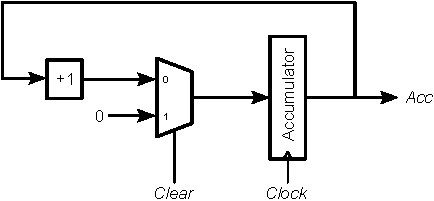
\includegraphics[width=.9\textwidth]{counter4bitaccclr}\\
    {\scriptsize Clear asserted: load 0}
  \end{column}
  \begin{column}{.33\textwidth}
    \centering
    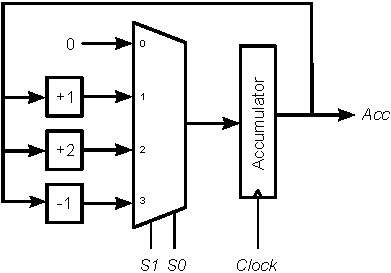
\includegraphics[width=.9\textwidth]{accum02bd}\\
    {\scriptsize Clear, +1, +2, $-1$}
  \end{column}
  \begin{column}{.33\textwidth}
    \centering
    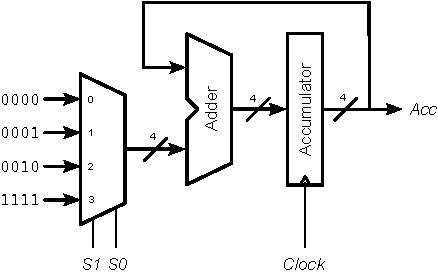
\includegraphics[width=.9\textwidth]{accum03bdx}\\
    {\scriptsize One adder, mux picks the operand}
  \end{column}
  \end{columns}
  \vspace{2mm}
  \begin{itemize}\small\itemsep2pt
    \item A mux in the feedback path changes the counting sequence. The single-adder version needs less hardware for the same functions.
  \end{itemize}
\end{frame}

\begin{frame}{Example: Multifunction Counter}
  \begin{columns}[c]
  \begin{column}{.4\textwidth}
    \centering
    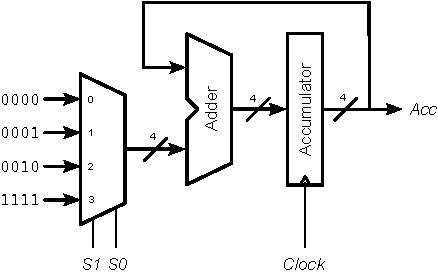
\includegraphics[width=.95\textwidth]{accum03bdx}\\[1mm]
    {\scriptsize The single-adder multifunction counter}\\[2mm]
    \scriptsize\striped
    \begin{tabular}{@{}cc|l@{}}
      \toprule
      $S_1$ & $S_0$ & Function \\
      \midrule
      0&0&Hold \\ 0&1&Add 1 \\ 1&0&Add 2 \\ 1&1&Subtract 1 \\
      \bottomrule
    \end{tabular}
  \end{column}
  \begin{column}{.58\textwidth}
    \centering\small\striped
    \begin{tabular}{@{}c|cc|l|c@{}}
      \toprule
      Clk & $S_1$ & $S_0$ & Function & $Q$ \\
      \midrule
      0 & -- & -- & initial & 0000 \\
      1 & 0 & 1 & Add 1 & 0001 \\
      2 & 0 & 1 & Add 1 & 0010 \\
      3 & 1 & 0 & Add 2 & 0100 \\
      4 & 1 & 1 & Subtract 1 & 0011 \\
      \bottomrule
    \end{tabular}
    \begin{itemize}\small\itemsep3pt
      \item Start at $Q = 0000$; control sequence $S_1S_0 = 01, 01, 10, 11$.
      \item After four pulses $Q = 0011_2 = 3$.
      \item The function can change on every pulse; one adder serves all operations.
    \end{itemize}
  \end{column}
  \end{columns}
\end{frame}

\begin{frame}{Timers}
  \begin{columns}[c]
  \begin{column}{.45\textwidth}
    \centering
    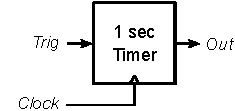
\includegraphics[width=.5\textwidth]{timer1sec_tl}\hspace{2mm}
    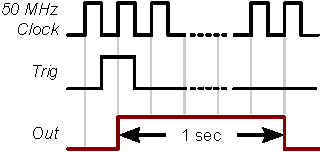
\includegraphics[width=.45\textwidth]{timer1sec_td}\\[2mm]
    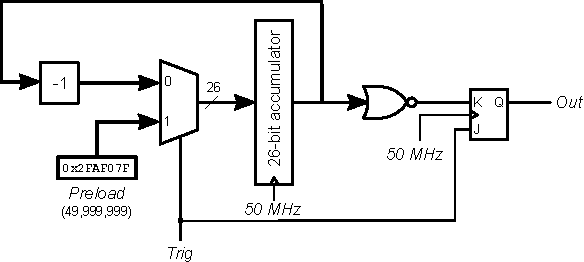
\includegraphics[width=.95\textwidth]{timer1sec_sc}
  \end{column}
  \begin{column}{.53\textwidth}
    \begin{itemize}\small\itemsep3pt
      \item A \alert{timer} gives a pulse of set duration: a one-shot (monostable).
      \item 1 s at 50 MHz: on \textit{Trig}, load a 26-bit accumulator with $50\,000\,000 - 1$ and set the JK flip-flop. It counts down; at zero a NOR gate resets the flip-flop.
    \end{itemize}
    \[ \text{Preload} = \text{Delay}\times\text{Frequency} - 1 \]
  \end{column}
  \end{columns}
\end{frame}

\begin{frame}{Prescaler}
  \begin{columns}[c]
  \begin{column}{.5\textwidth}
    \centering
    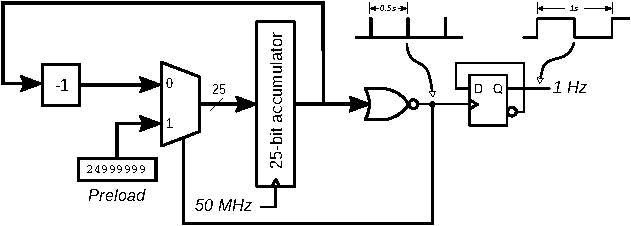
\includegraphics[width=\textwidth]{prescaler_sc}
  \end{column}
  \begin{column}{.48\textwidth}
    \begin{itemize}\small\itemsep3pt
      \item A \alert{prescaler} derives a slow time base from a fast clock.
      \item 25-bit counter loaded with $25\,000\,000 - 1$ and decremented each cycle. At zero a NOR gate pulses and reloads it: one pulse every 0.5 s, i.e.\ 2 Hz.
      \item The pulses are very asymmetric. A D flip-flop in toggle mode gives a symmetric \alert{1 Hz}, 50\% duty cycle.
      \item A \emph{programmable} prescaler takes its preload from a control circuit.
    \end{itemize}
  \end{column}
  \end{columns}
  \vspace{2mm}
  {\small Timers and prescalers need big counters. When timing is not critical, a 555 timer (monostable or astable) is cheaper.}
\end{frame}

\begin{frame}{Back to the Opening Question}
  \begin{block}{Serial links use shift registers}
    \small A USB-like link sends bits one after another on a few wires. The sender loads a word in parallel and shifts it out serially (\alert{PISO}). The receiver shifts the bits in (\alert{SIPO}) and reads the whole word in parallel. Two or three wires carry data and clock, yet thousands of bytes are exchanged.
  \end{block}
\end{frame}

%===============================================================================
\section{Summary}
%===============================================================================

\begin{frame}{Summary}
  \begin{itemize}\itemsep3pt\small
    \item An $n$-bit \alert{data register} is $n$ flip-flops sharing a clock and, optionally, a clear and a load enable.
    \item A \alert{shift register} shifts the stored word one position per clock. Its main use is serial--parallel conversion (SIPO, PISO).
    \item A \alert{ring counter} recirculates a single 1; a \alert{Johnson counter} feeds back the complement and visits $2n$ states.
    \item An \alert{LFSR} XORs selected taps back to the input and generates a pseudo-random sequence.
    \item An \alert{accumulator} with an incrementer is a counter; a timer or prescaler is a loadable down-counter with a terminal-count detector.
  \end{itemize}
  \begin{block}{Looking ahead}
    Chapter 12 builds counters directly from flip-flops, circuits that produce an ordered sequence of states for counting, dividing and timing.
  \end{block}
\end{frame}

\end{document}
